\begin{apendicesenv}
\partapendices

\chapter{Published papers}
\label{chap:Artigo}
    Below are the papers published since the beginning of this research. The first and second article presented refers to the publication made about this PhD, with mixed results of the techniques used in the master's dissertation \cite{Dissertacao} and this thesis. The third and forth articles presented refer to publications made during the master's dissertation, but which express the techniques used in this thesis project. 

\section{Large-deviation quantification of boundary conditions on the Brazil nut effect}
\label{appendix:BNE}
    This paper was published on the Physical Review E, and it is one of the main themes of this thesis, referring to chapter \ref{chap:BNE}. It is an A2 magazine according to the CAPES \textit{qualis} classification and has an impact factor of 2.529.

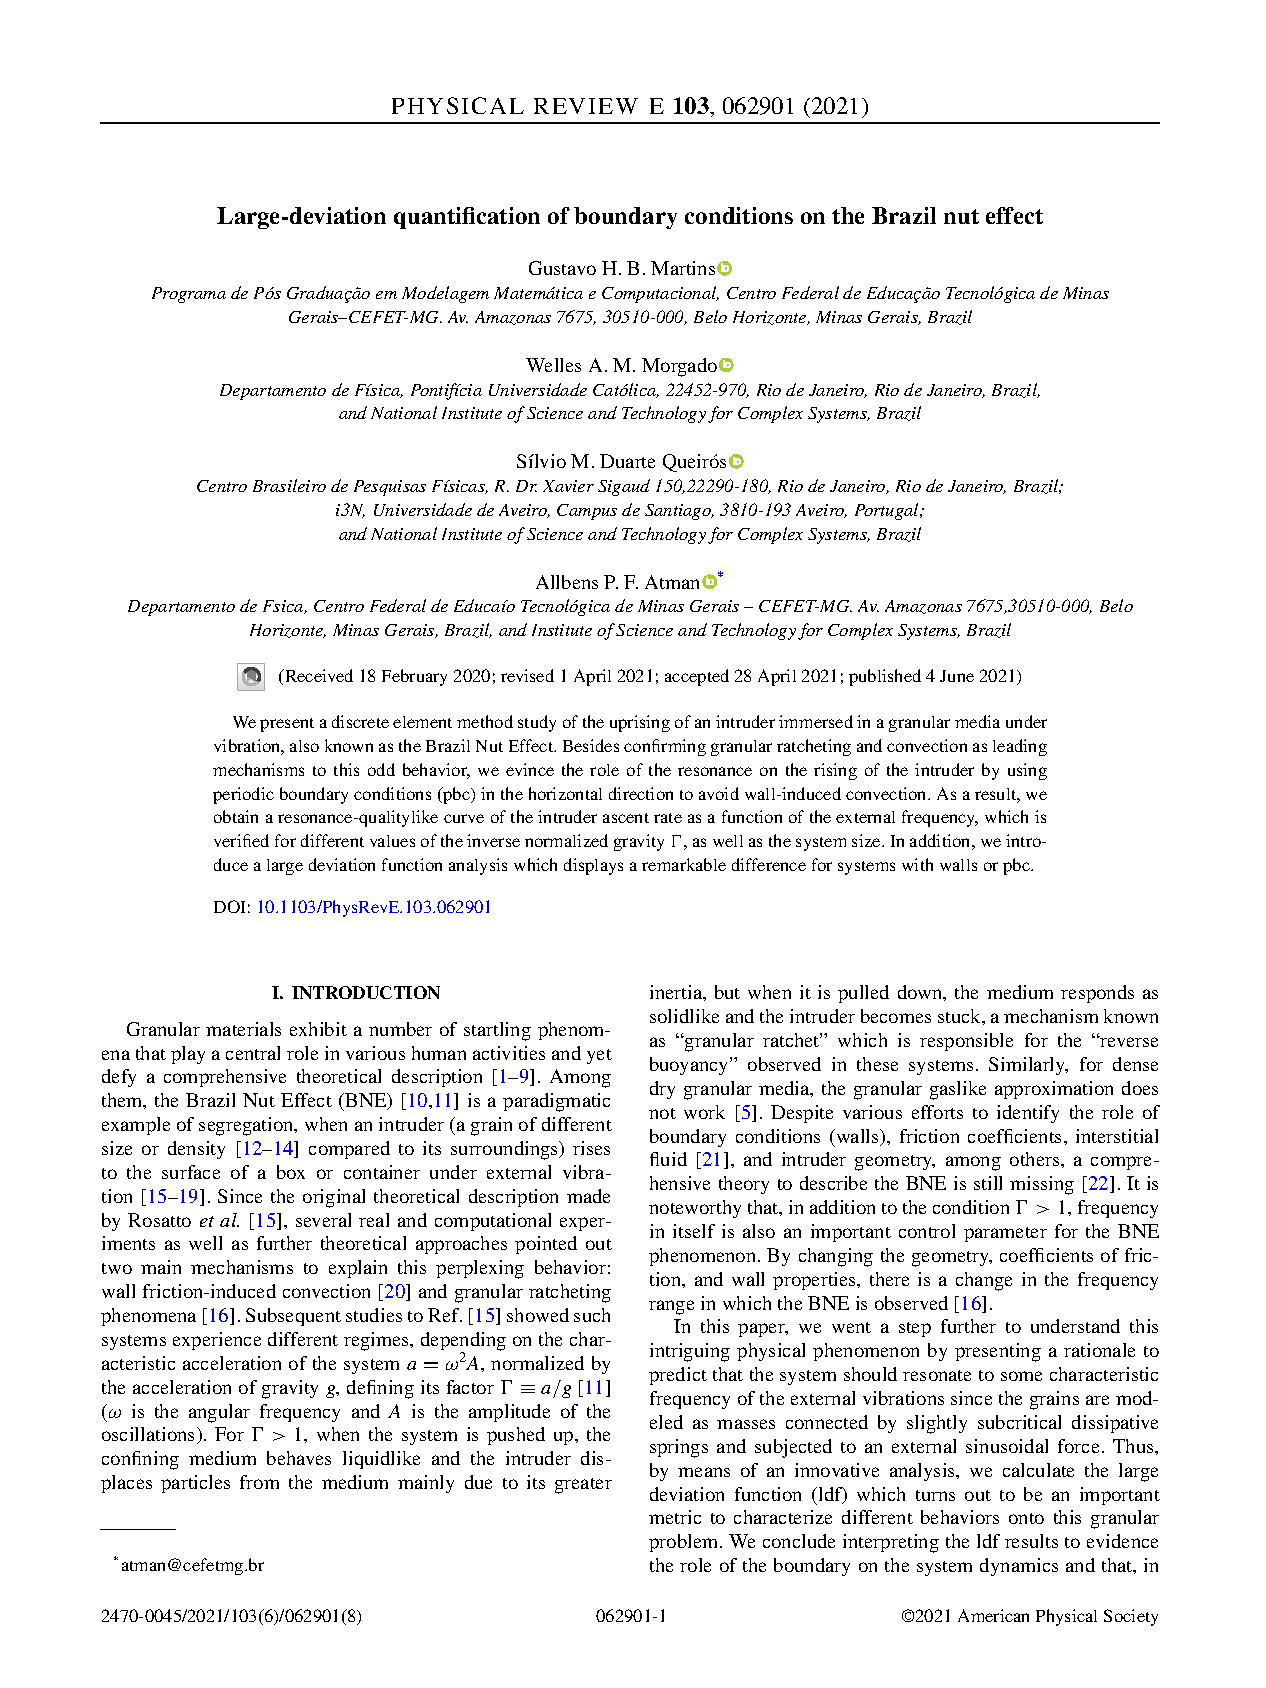
\includepdf[pages=-]{08-apendice/ArtigoPRE.pdf}

\section{Methods of parallel computation applied on granular simulations}
    This paper was published at the four-year conference Powders \& Grains 2017 - 8$^\textrm{th}$ edition, which is the largest conference on granular materials.

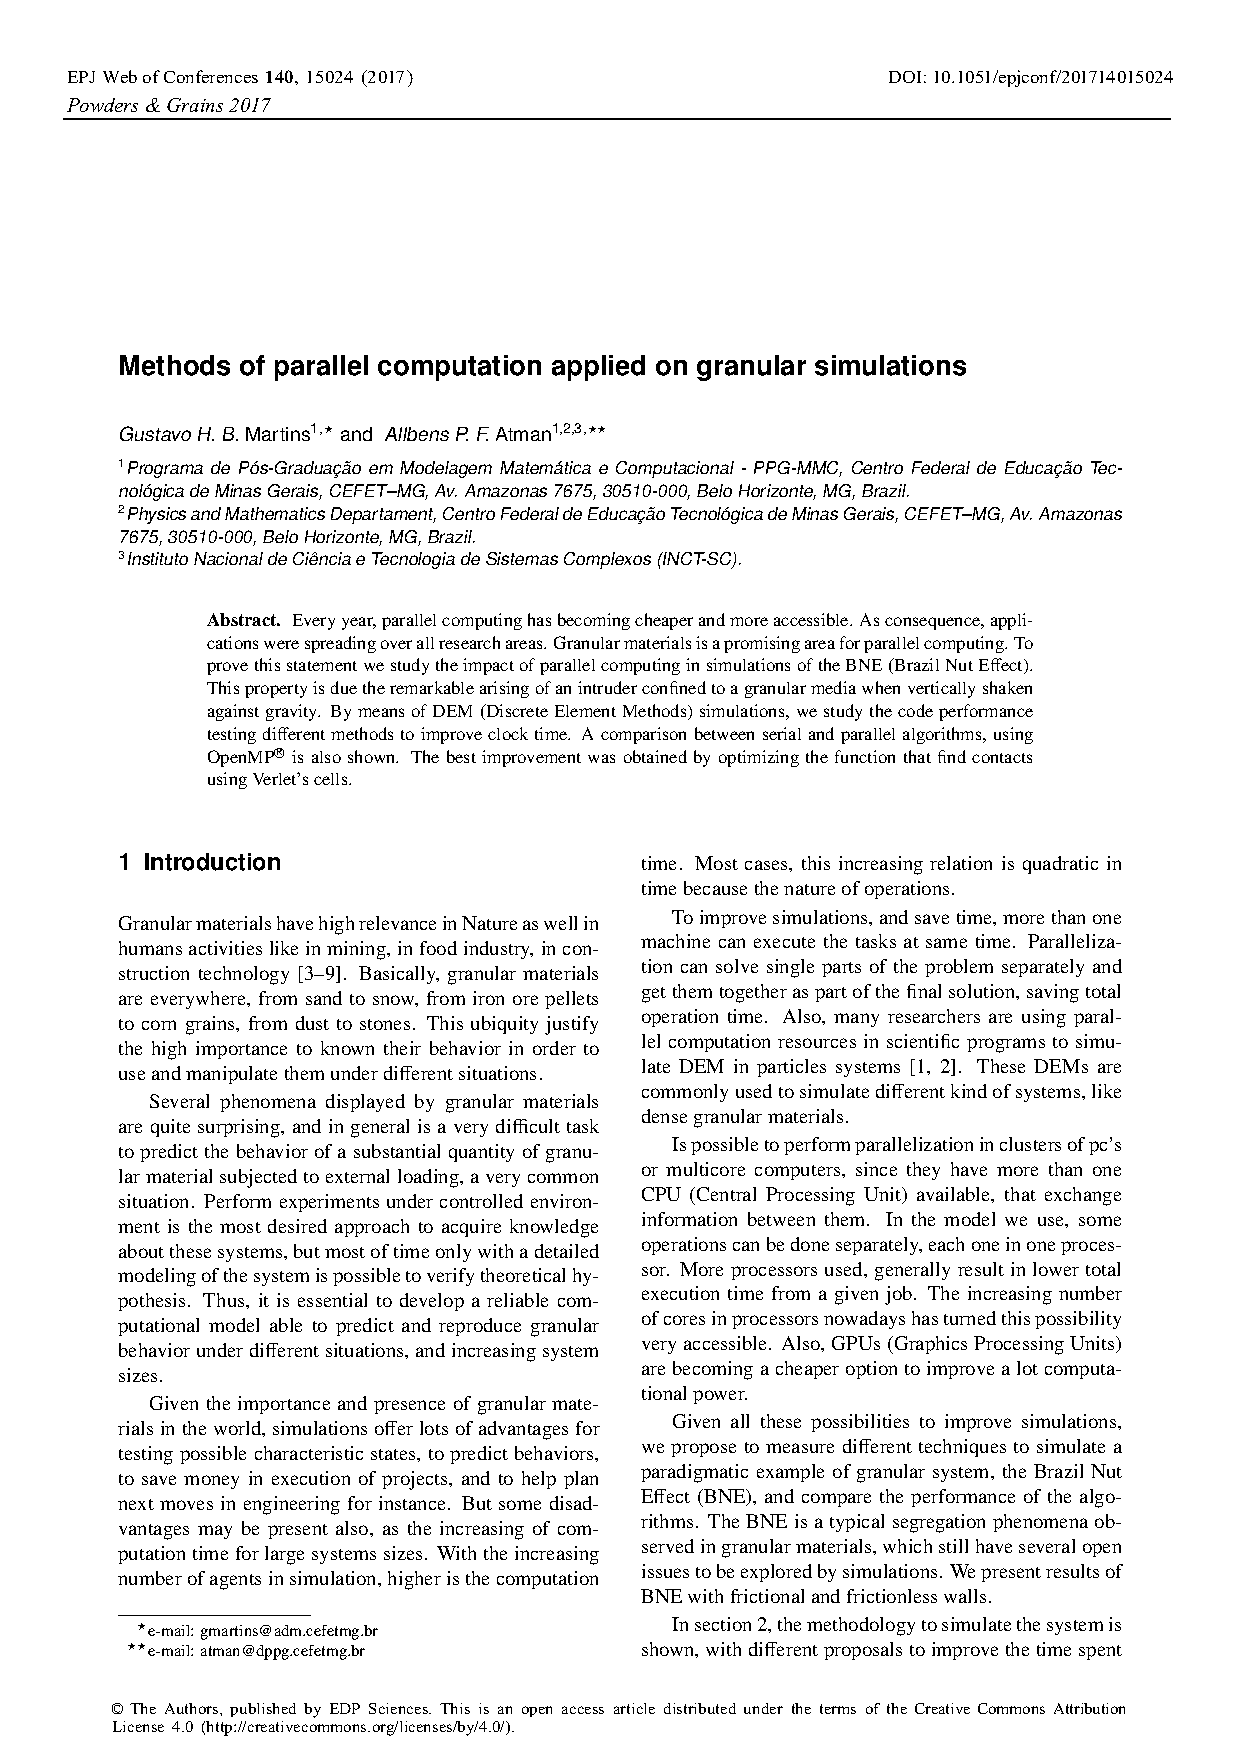
\includepdf[pages=-]{08-apendice/ArtigoPG2017.pdf}

\section{Mechanical properties of inclined frictional granular layers}
%    Este artigo foi publicado na \textit{Granular Matter}, uma das maiores revistas sobre material granular e é uma revista A2 segundo a classificação \textit{qualis} da CAPES e possui fator de impacto de $1,762$.

    This paper was published at Granular Matter, one of the largest magazines on granular material and is an A2 magazine according to the CAPES \textit{qualis} classification and has an impact factor of 2.652.

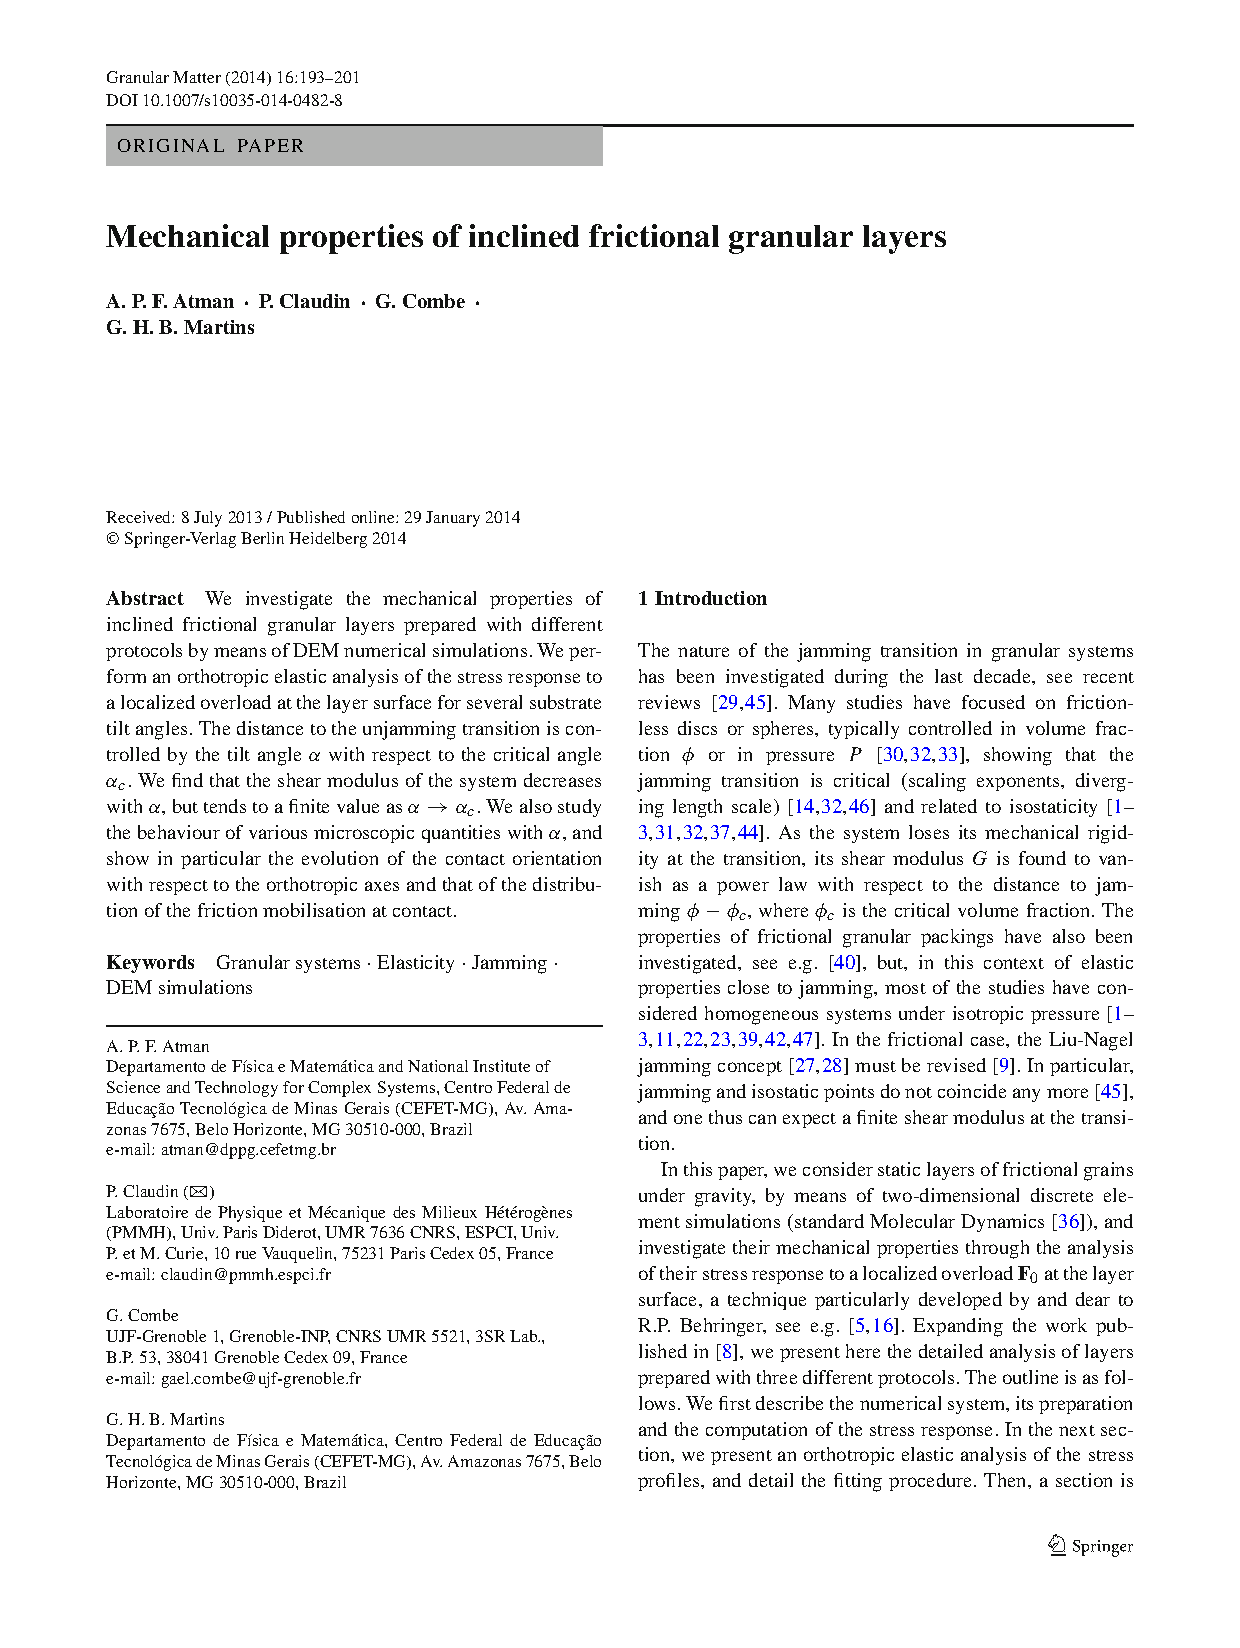
\includepdf[pages=-]{08-apendice/ArtigoGM.pdf}

\section{Non-Gaussian behavior in jamming / unjamming transition in dense granular materials}
%    Este artigo foi publicado no quatrienal do congresso \textit{Powders \& Grains 2013}, que é o maior congresso sobre materiais granulares, e que estava em sua 7ª edição.

    This paper was published at the four-year conference Powders \& Grains 2013 - 7$\textrm{th}$ edition, which is the largest conference on granular materials.

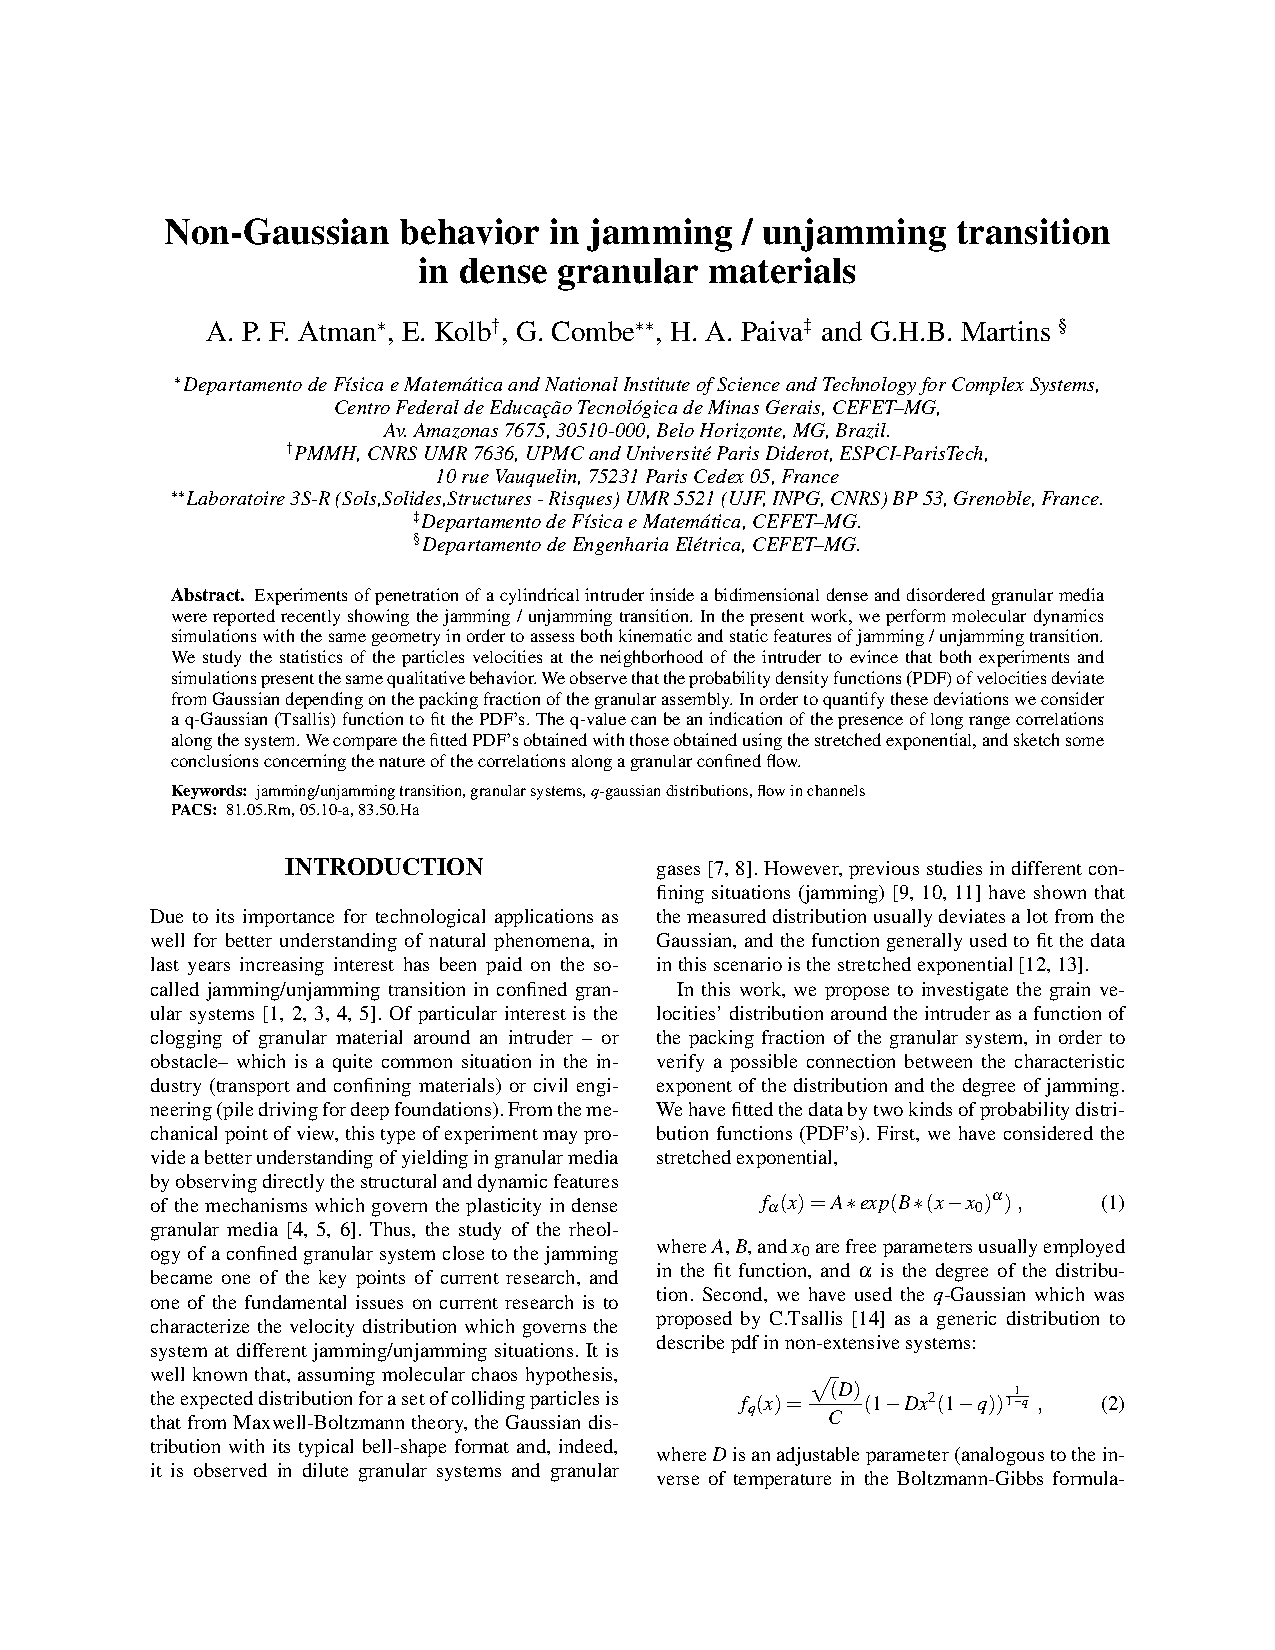
\includepdf[pages=-]{08-apendice/ArtigoPG2013.pdf}

\chapter{Codes}
%    Coloquei os códigos utilizados para este projeto de tese em um GIT para a maior comodidade e facilidade do acesso. O endereço eletrônico é \url{https://github.com/BoscoWarhammer/Doutorado}.

    I have placed the codes used in this thesis project in a GIT for greater convenience and ease access. The electronic address is \url{https://github.com/BoscoWarhammer/Doutorado}.

\chapter{Turbulence}
\label{chap:Turbulence}
\section{Turbulent steady-state regime}
    There are several turbulence models to be addressed in a fluid approach. In this work we choose the Prandtl turbulence model and the term turbulent viscosity is presented as in the following equation:
\begin{equation}
    \begin{array}{l}
        \nu_{t} = l^2\left|\dot{\gamma}\right|, \textrm{in other words,} \\
        \nu_{t} = l^2\left|\frac{\partial u_{x}}{\partial z}\right|,
    \end{array}
    \label{equ:viscosidade_turbulenta}
\end{equation}
where $\nu_{t}$ is the turbulent model, $l$ is the characteristic vortex turbulence length, $\dot{\gamma}$ is the fluid strain rate, $u_x$ is the fluid velocity in the flow direction and $z$ is the gravity direction.

    Fluid shear controls some fluid characteristics, such as the flow regime. The equation that governs shear is the equation:
\begin{equation}
    \tau = \rho^{f}\left(\nu+l^{2}\left|\frac{\partial u_{x}}{\partial z}\right|\right)\frac{\partial u_{x}}{\partial z},
    \label{equ:cisalhamento}
\end{equation}
where $\tau$ is the shear flow, $\rho^f$ is the fluid density, $\nu$ is the intrinsic fluid viscosity, $l^2 \left|\frac{\partial u_{x}}{\partial z}\right|$ is the viscosity term that emulates average turbulence\footnote{RANS - Reynolds average Navier-Stokes: time average equations of the motion for fluid flow.} and $\frac{\partial u_{x}}{\partial z}$ is the fluid strain rate tensor and is equivalent to the Equation \ref{equ:taxa_deformacao}.

    For the mixture of fluid and granular, we take the characteristic length of the turbulence always above the static layers of the granular material, and therefore assume the behavior of the turbulent characteristic length described by the Equation \ref{equ:comprimento_turbulencia}, proposed by van Driest \cite{Numerical_simulation_of_turbulent_sediment_transport}:
\begin{subequations}
    \begin{empheq}[left={l(z_{b}) =}\empheqlbrace]{align}
        & 0 & \textrm{se } z \leq z_{b}, 
        \label{equ:comprimento_turbulencia_granular} \\
        & \kappa (z -z_{b})\left[1-e^{-\left(z -z_{b}\right)\frac{u_{*}}{\nu \mathcal{R}_{vD}}} \right] & \textrm{if } z > z_{b},
        \label{equ:comprimento_turbulencia_fluido}
    \end{empheq}
    \label{equ:comprimento_turbulencia}
\end{subequations}
where $l(y_{b})$ is the turbulent characteristic length, $\kappa \simeq$ 0.4 is the von Karman's constant, $z$ is the height of the fluid, $z_{b}$ is the position of the granular bed, $u_{*}$ is the characteristic shear velocity imposed at the top of the fluid, $\nu$ is the viscosity of the fluid and $\mathcal{R}_{vD} \simeq$ 26 is the van Driest's Reynolds number \cite{Numerical_simulation_of_turbulent_sediment_transport}. However, other characteristic lengths of turbulence were taken into account and are described in the references \cite{Numerical_simulation_of_turbulent_sediment_transport, Maurin-Tese}. 

    We wish to find the final velocity profile that does not change in time, like equation \ref{equ:dudt0}, and by consequence, also the shear profile does not change in space, like Equation \ref{equ:dtaudz0}. Again, if Equation \ref{equ:dtaudz0} do not change in space, then $\tau$ is a constant everywhere, making Equation \ref{equ:viscous_steady0} to be a constant. Making explicit the change of velocity in function of space ($\partial u/\partial z$), we get Equation \ref{equ:turbulent_steady0}, with $\partial u/\partial z \geq 0$. It means that Equation \ref{equ:turbulent_steady0} must be integrated according to $z$ to get the velocity profile of the fluid.
\begin{equation}
    \frac{\partial u}{\partial z} = \frac{-\nu+\sqrt{\nu^2+4l^2\tau/\rho}}{2l^2},
    \label{equ:turbulent_steady0}
\end{equation}
with $\tau = \rho {u_{*}}^{2}$ imposed on top, and it is constant everywhere. In the case of this this equation, the solution is not analytical, and we computed it through Runge-Kutta 4$^{th}$ order solution\footnote{In section \ref{sec:RK} we are presenting the Runge-Kutta method to solve a ordinary differential equation numerically.}, presented in equation \ref{equ:RK}. Figure \ref{fig:turbulent_steady} shows us the shape of the normalized solution to equation \ref{equ:turbulent_steady0}.

    To best characterize the solution of equation \ref{equ:turbulent_steady0}, we are going to looking at the two asymptotic behaviors it has: one lower, at $z\to 0$, and the other at $z\to\infty$. When $z\to 0$, the mixing length tends to zero because the exponential tends to one, killing the contribution of the mixing length. So, for small size, compared with the characteristic length of the fluid ($u_*/\nu$), the fluid behave as a viscous fluid. Then the asymptotic behavior near to the wall:
\begin{equation}
    \lim_{z \to 0} \frac{\partial u}{\partial z} = \frac{u_*^2}{\nu},
\end{equation}
we get equation \ref{equ:viscous_steady0}, because we are working with a very small mixing length, given by equation \ref{equ:comprimento_turbulencia}. We already know this solution, and it is showed in equation \ref{equ:viscous_steady1}. On the other hand, the other asymptotic at $z\to\infty$, leads the mixing length to $\kappa z$ because the exponential tends to zero, having almost the full contribution of $\kappa z$, then the asymptotic equation to be analyzed is:
    \begin{equation}
        \lim_{z \to \infty} \frac{\partial u}{\partial z} = \frac{u_*}{\kappa z},
    \end{equation}
and the solution to this differential equation is, as next:
    \begin{equation}
        u^+ = \frac{1}{\kappa}\ln\left(\frac{z}{z_0}\right),
    \end{equation}
where $z_0=0.1\nu/u_*$ is the length that came from a perfect flat surface in a pure turbulent regime, and it is as if it scales with this perfect flat surface, although it faces a viscous sublayer.

\begin{figure}[H]
    \centering
    \parbox{0.495\textwidth}{
        \centering
        \includegraphics[width= 0.45\textwidth]{04-figuras/turbulent_steady_velocity.tikz}
        \subcaption{Normalized velocity of viscous-turbulent steady-state profile.}
        \label{fig:turbulent_steady_velocity}
    }
    \parbox{0.495\textwidth}{
        \centering
        \includegraphics[width= 0.45\textwidth]{04-figuras/turbulent_steady_shear.tikz}
        \subcaption{Normalized shear of viscous-turbulent steady-state profile.}
        \label{fig:turbulent_steady_shear}
    }
    \caption[Steady-state numerical solution for viscous-turbulent fluid profiles.]{Velocity and shear steady-state profiles for the viscous-turbulent fluid. The red continuous line is the solution to van Driest's equation. The dashed blue line is the viscous asymptotic regime, like in the previous section \ref{sec:viscous_steady}. The dotted blue line is the pure turbulent behavior, which corresponds to the normalized velocity profile: $u^+=\kappa^{-1}\ln(z^+/0.1)$.}
    \label{fig:turbulent_steady}
\end{figure}

    As expected, there is a viscous sublayer regime, combined with a transitional layer to the turbulent behavior. The profile of the viscous regime is linear profile, while the turbulent regime has an asymptotic to logarithmic function. Again, as we are not limited by an upper boundary, the fluid has an infinity characteristic length in the steady-state regime.

        \subsection{A little bit more complicated mixing length}
    This complication on mixing length will give us a different approach to the temporal evolution of the fluid equation. To the steady state, it was built to give approximately same result as equation \ref{equ:comprimento_turbulencia}. Equation \ref{equ:OD_mixing_length} has been proposed by Orencio Durán in \cite{Numerical_simulation_of_turbulent_sediment_transport}.

\begin{equation}
    \frac{\partial l}{\partial z} = \kappa \left[1-e^{-\sqrt{\frac{1}{R_c}\left(\frac{ul}{\nu}\right)}}\right],
    \label{equ:OD_mixing_length}
\end{equation}
where $R_c = 7$ is a Reynolds number that control the response of the equation to achieve the best comparison of the velocity profile obtained by integration of this equation to the one obtained using the van Driest's expression \ref{equ:comprimento_turbulencia}. With equation \ref{equ:turbulent_steady0} and \ref{equ:OD_mixing_length}, we can write a system and solve by Runge-Kutta method extended to first-order ODEs, as shown in \ref{sec:RK}.

\end{apendicesenv}
